\section{Auswertung}
\label{sec:Auswertung}
\subsection{Verifizieren der Linsengleichung}
Um das Abbildungsgesetz sowie die Linsengleichung (Gleichungen \eqref{eqn:V} und \eqref{eqn:D}) zu verifizieren sind die dafür relevanten Messwerte in Tabelle \ref{tab:VdA} aufgetragen. Die Gegenstandsgröße des Perl L beträgt
\begin{equation}
  G = 3.0 \cdot 10^{-2} \, \text{m} \ .
\end{equation}
Die Vergrößerungen werden entsprechen $V_1 = \frac{b}{g}$ und $V_2 = \frac{B}{G}$ berechnet und deren relative Messabweichung in der Tabelle \ref{tab:VdA} aufgelistet. Die Brennweite zu den Bildweiten $b$ sowie Gegenstandsweiten $G$ werden mittels der Linsengleichung (Gleichung \eqref{eqn:D}) berechnet und ebenfalls in der Tabelle aufgelistet.
\begin{table}
  \centering
  \begin{tabular}{c c c | c | c c c c}
    \toprule
    $g / 10^{-2}$ m & $b / 10^{-2}$ m & $B / 10^{-3}$ m & $f / 10^{-2}$ m & $V_1$ & $V_2$ & $\left\lvert \frac{V_1 - V_2}{V_1} \right\rvert / \% $\\
   \midrule
    25.0 & 15.6 & 2.0 & 10.4 & 0.62   & 0.66	& 6.6 	\\
    24.0 & 16.4 & 2.0 & 10.2 & 0.68   & 0.66	& 3.0	\\
    23.0 & 16.8 & 2.2 & 10.3 & 0.73   & 0.73	& 0.0	\\
    22.0 & 17.6 & 2.3 & 10.2 & 0.80   & 0.77	& 3.8	\\
    21.0 & 18.4 & 2.7 & 10.2 & 0.88   & 0.90	& 2.3	\\
    20.0 & 19.3 & 2.7 & 10.2 & 0.97   & 0.90	& 7.2	\\
    19.0 & 20.5 & 3.1 & 10.1 & 1.08   & 1.03	& 4.7	\\
    18.0 & 21.4 & 3.4 & 10.2 & 1.18   & 1.13	& 4.2	\\
    17.0 & 23.1 & 4.2 & 10.2 & 1.35   & 1.40	& 3.7	\\
    16.0 & 25.1 & 4.7 & 10.2 & 1.56   & 1.57	& 0.6	\\
    15.0 & 29.2 & 5.7 & 10.1 & 1.94   & 1.90	& 2.1	\\
    \midrule
    \multicolumn{3}{r|}{(Mittelwert $\pm$ Fehler des Mittelwertes)}&(\num {10.2 +- 0.1}) & & & (\num{3.5 +- 0.7})\\
    \bottomrule
  \end{tabular}
  \caption{Messwerte und berechnete Größen zur Verifizierung des Abbildungsgesetzes und Linsengleichung}
  \label{tab:VdA}
\end{table}
Das Abbildungsgesetz wurde durch die Messung bestätig, da die Werte einen Fehler von durchschnittlich 3.5 \% aufweisen. Dies liegt innerhalb des Toleranzbereichs der Messunsicherheit bei den Versuchen im Praktikum. Die Linsengleichung ist ebenso verifiziert worden da die durchschnittliche Brennweite einen Fehler von 2\% aufweist gegenüber der Herrstellerangabe von
\begin{equation}
  f_\text{Hersteller} = 1.0 \cdot 10^{-1} \, \text{m} \ .
  \label{eqn:fHer1}
\end{equation}
\subsection{Bestimmung einer bekannten sowie unbekannten Brennweite}
Die Brennweite der bekannten Linse wurde bereits im vorherigen Kapitel mit Hilfe der Linsengleichung bestimmt. Zusätzlich wird die Brennweite mit Hilfe eines Plots bestimmt. Dafür werden die Gegenstandsweiten auf die y-Achse des Koordinatensystems aufgetragen werden und mit den entsprechenden Bildweiten, welche auf der x-Achse aufgetragen sind, verbunden werden. Aus dem Schnittpunkt der Geraden lässt sich die Brennweite der Linse ablesen. Aus Abbildung \ref{fig:fibek} wird die Brennweite
\begin{equation}
  f_\text{abgelesen} = (\num{9.8 +- 0.4}) 10^{-2} \, \text{m}
  \label{eqn:fbek}
\end{equation}
abgelesen.
\begin{figure}
  \centering
  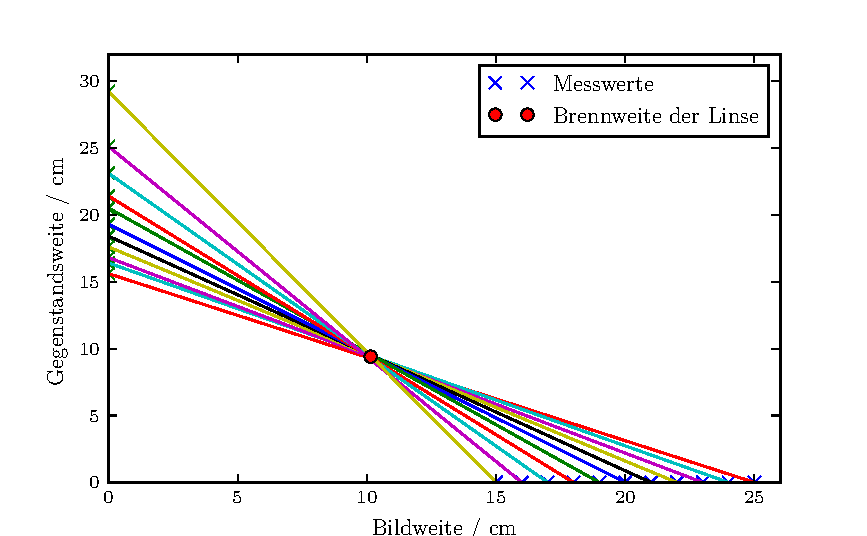
\includegraphics[height=8cm]{bekannt.pdf}
  \caption{Brennweite einer bekannten Linse}
  \label{fig:fibek}
\end{figure}
Die Messung wird für eine Linse mit unbekannter Brechkraft wiederholt. Die Messdaten und die Brennweiten sind in Tabelle \ref{tab:funb} aufgetragen.
\begin{table}
  \centering
  \begin{tabular}{c c| c}
    \toprule
    $b/10^{-2}$ m & $g/10^{-2}$ m & $f/10^{-2}$ m\\
    \midrule
	40.0	& 15.0	& 9.2	\\
	39.0	& 15.1	& 9.2	\\
	38.0	& 15.3	& 9.2	\\
	37.0	& 15.5	& 9.2	\\
	36.0	& 15.8	& 9.1	\\
	35.0	& 16.3	& 9.0	\\
	34.0	& 16.6	& 9.0	\\
	33.0	& 17.0	& 9.0	\\
	32.0	& 17.5	& 8.9	\\
	31.0	& 17.8	& 8.8	\\
	30.0	& 18.4	& 8.8	\\
    \midrule
    	\multicolumn{2}{r|}{(Mittelwert $\pm$ Fehler des Mittelwertes)}&(\num {9.0 +- 0.1})\\
    \bottomrule
  \end{tabular}
  \caption{Gemessene Bild-, Gegenstandsweite und errechnete Brennweite einer unbekannten Linse}
  \label{tab:funb}
\end{table}
Aus dem Diagramm \ref{fig:fiunb} lässt sich eine Brennweite von
\begin{equation}
  f_\text{unbekannt} = (\num{11.9 +- 2.3}) \, \text{m}
  \label{eqn:unb}
\end{equation}
ablesen.
\begin{figure}
  \centering
  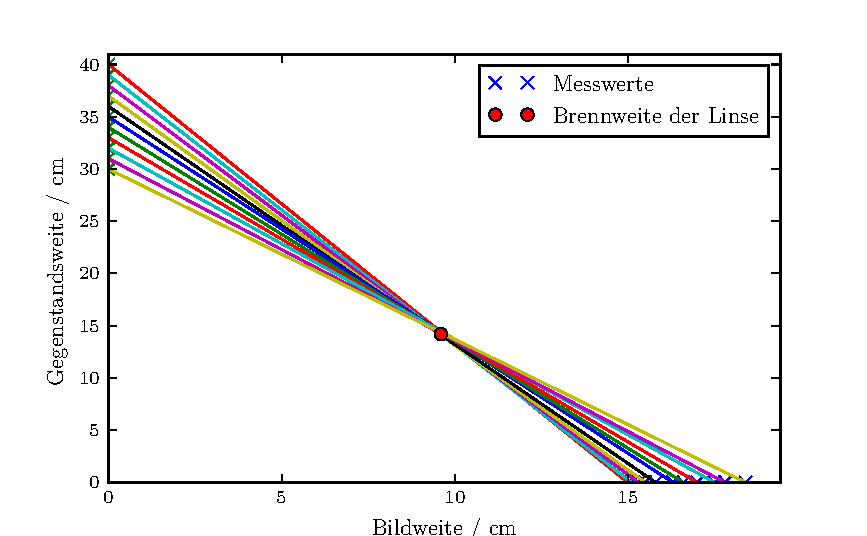
\includegraphics[height=8cm]{unbekannt.pdf}
  \caption{Brennweite einer unbekannten Linse}
  \label{fig:fiunb}
\end{figure}
\subsection{Verfahren nach Bessel}
Die entsprechenden Messdaten zu dem Versuch sind in Tabelle \ref{tab:ffw} zu finden. Dabei wird die Brennweite nach Formel \eqref{eqn:tbes} berechnet, wobei der Abstand $d = g - b$ und die Gegenstandsweite als $g = e - b$ demenstsprechend definiert ist.
\begin{table}
  \centering
  \begin{tabular}{c c c | c c}
    \toprule
    $e$ / $10^{-2}$ m & $g_1$ / m & $g_2$ / m & $f_1$ / $10^{-2}$ m & $f_2$ / $10^{-2}$ m\\
    \midrule
	100.0	& 11.5	& 89.3	& 10.18	& 9.56	\\
	97.5	& 11.5	& 86.9	& 10.14	& 9.45	\\
	95.0	& 11.6	& 84.4	& 10.18	& 9.42	\\
	92.5	& 11.6	& 81.6	& 10.15	& 9.62	\\
	90.0	& 11.7	& 79.1	& 10.18	& 9.58	\\
	87.5	& 11.7	& 76.5	& 10.14	& 8.62	\\
	85.0	& 11.8	& 75.1	& 10.16	& 7.75	\\
	82.5	& 11.9	& 73.6	& 10.18	& 9.94	\\
	80.0	& 11.9	& 68.9	& 10.13	& 9.56	\\
	77.5	& 12.1	& 66.4	& 10.21	& 9.51	\\
   \midrule
		&	&	& \num{10.17 +- 0.01} & \num{9.30 +- 0.17} \\
   \bottomrule
  \end{tabular}
  	\caption{Brennweite von weißem Licht}
  \label{tab:ffw}
\end{table}
Aus der Mittelung der einzelnen Messwerte erhält ??man?? durch das Bessel-Verfahren eine experimentell bestimmte Brennweite für weißes Licht von
\begin{equation}
  f_\text{exp} = (\num{9.73 +- 0.13}) 10^{-2} \, \text{m} \ .
  \label{eqn:fexp}
\end{equation}
Wenn der Fehler aus den Zwischensummen der einzelnen Brennweiten $f_1$ und $f_2$ genommen wird beträgt er
\begin{equation}
  \Delta \overline{f_\text{exp}} = 0.43 \cdot 10^{-2} \, \text{m}
  \label{eqn:fehlerkomisch}
\end{equation}
Für den Versuch wurde eine Linse mit einer Brennweite von
\begin{equation}
  f_\text{Hersteller} = 10 \cdot 10^{-2} \, \text{m} \
  \label{eqn:fHer}
\end{equation}
verwendet.
Anschließend wird die Brechkraft von farbigem Licht bestimmt. Dazu wird zunächst ein roter und anschließend ein blauer Farbfilter vor die Lampe gespannt.
\begin{table}
  \centering
  \begin{tabular}{c | c c c || c c c}
    \toprule
    $e$ / m & $g_\text{rot} / 10^{-2}$ m & $b_\text{rot} / 10^{-2}$ m & $f_\text{rot} / 10^{-2}$ m & $g_\text{blau} / 10^{-2}$ m & $b_\text{blau} / 10^{-2}$ m & $f_\text{blau} / 10^{-2}$ m \\
    \midrule
    100	& 89.3	& 10.7	& 9.56&	89.3 & 10.7 & 9.56	\\
    90	& 79.1	& 10.9	& 9.58& 79.3 & 10.7 & 9.43	\\
    80	& 68.8	& 11.2	& 9.63& 69.0 & 11.0 & 9.49	\\
    70	& 58.5	& 11.5	& 9.61& 58.6 & 11.4 & 9.54	\\
    60	& 48.0	& 12.0	& 9.60& 48.4 & 11.6 & 9.42	\\
    \bottomrule
  \end{tabular}
  \caption{Brennweite von rotem und blauem Licht}
  \label{tab:fbesslf}
\end{table}
Aus Tabelle \ref{tab:fbesslf} ergibt sich für rotes Licht eine Brennweite von
\begin{equation}
  f_\text{rot} = (\num{9.60 +- 0.01}) \, 10^{-2} \, \text{m}
  \label{eqn:frot}
\end{equation}
und für blaues Licht eine Brennweite von
\begin{equation}
  f_\text{blau} = (\num{9.49 +- 0.03}) \, 10^{-2} \, \text{m} \ .
  \label{fblau}
\end{equation}

\subsection{Verfahren nach Abbe}
Es sollen die Hauptebene und die Brennweite mit Hilfe der Formeln \eqref{eqn:g'} und \eqref{eqn:b'} bestimmt werden. Es wird eine Zerstreuungslinse und Fokussierlinse jeweils von 10 $10^{-2}$ m Brennweite im Abstand von
\begin{equation}
  d = 6 \cdot 10^{-2} \, \text{m}
  \label{eqn:d}
\end{equation}
verwendet. Die Gegenstandsgröße des Objektes beträgt
\begin{equation}
  G = 3 \cdot 10^{-2} m \ .
  \label{eqn:G}
\end{equation}
Die Messwerte sind in Tabelle \ref{tab:mabbe} aufgetragen.
\begin{table}
  \centering
  \begin{tabular}{c c c c}
    \toprule
    	$g$ / $10^{-2}$ m & $b$ / $10^{-2}$ m & $B$ / $10^{-2}$ m & $V$ \\
    \midrule
	104.4	& 15.6	& 14.8	& 4.93	\\
	99.0	& 16.0	& 13.5	& 4.50	\\
	93.7	& 16.3	& 12.5	& 4.17	\\
	88.3	& 16.7	& 11.5	& 3.83	\\
	82.7	& 17.3	& 10.2	& 3.40	\\
	77.0	& 18.0	& 9.1	& 3.03	\\
	71.5	& 18.5	& 8.3	& 2.77	\\
	65.5	& 19.5	& 7.1	& 2.37	\\
	59.4	& 20.6	& 6.2	& 2.07	\\
	52.0	& 23.0	& 4.8	& 1.60	\\
    \bottomrule
  \end{tabular}
  \caption{Messwerte zur Bestimmung der Brennweite mittels Abbemethode}
  \label{tab:mabbe}
\end{table}
Es wird zunächst eine lineare Regression entsprechend Gleichung \eqref{eqn:g'} durchgeführt und die Fitparameter $f_\text{g}$ und $h$ ermittelt. Anhand derer kann ??man?? aus der Steigung des Graphens und den Schnittpunkten mit der Achse die Hauptebenen und die Brennweiten berechnen.
\begin{figure}
  \centering
    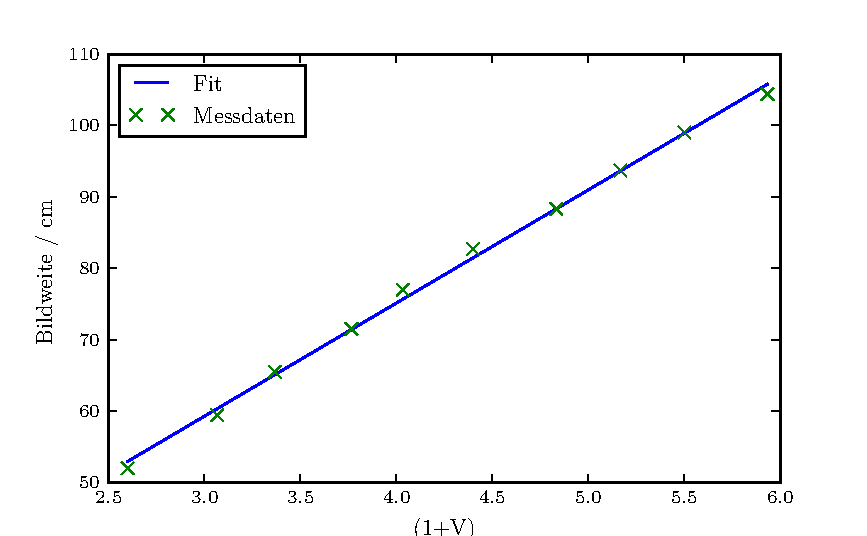
\includegraphics[height=8cm]{Abbe1.pdf}
  \caption{Bildweiten Fit}
  \label{fig:Gfit}
\end{figure}
Der Fit durch die Messwerte ist in Abbildung \ref{eqn:Gfit} zu sehen.
\begin{figure}
  \centering
  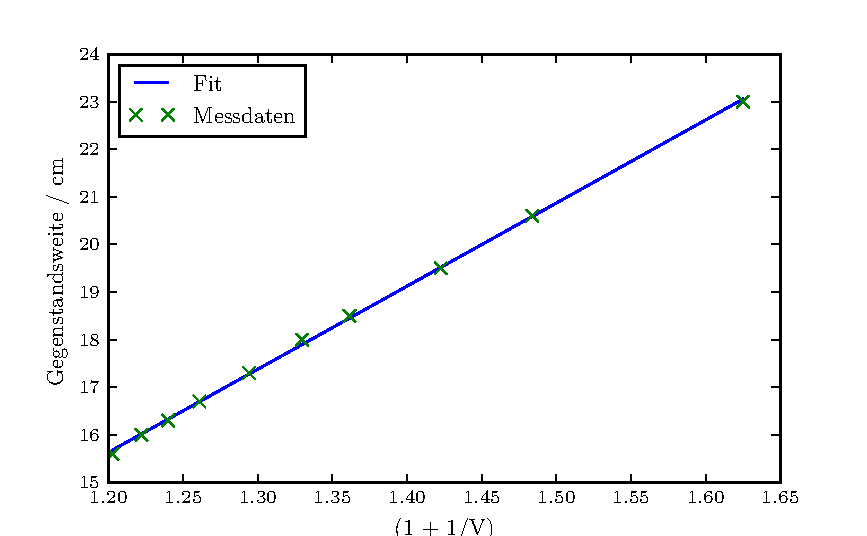
\includegraphics[height=8cm]{Abbe2.pdf}
  \caption{Gegenstandsweiten Fit}
  \label{fig:Bfit}
\end{figure}
Der Fit der Form von Gleichung \eqref{eqn:b'} ergibt die Brennweiten und die Lage der Hauptebenen
\begin{eqnarray}
  f_\text{g} &= (\num{ 15.9 +- 0.3}) \cdot 10^{-2} \, \text{m} \\
  f_\text{b} &= (\num{ 17.5 +- 0.1 }) \cdot 10^{-2} \, \text{m} \\
  h &= (\num{ 11 +- 1}) \cdot 10^{-2} \, \text{m} \\
  h' &= (\num{ -5.3 +- 0.2}) \cdot 10^{-2} \,\text{m}
  \label{eqn:abbedf}
\end{eqnarray}
Die theoretische Brennweite des Systems berechnet sich aus der Modifikation von Formel \eqref{eqn:D} um einen Korrekturfaktor zu
\begin{eqnarray}
  \frac{1}{f} &= \frac{1}{f_1} + \frac{1}{f_2} - \frac{d}{f_1 * f_2} \\
  f &= 16.6 \cdot 10^{-2} \, m \ .
  \label{tabbe}
\end{eqnarray}
